\chapter{虚拟实验室与评价协议}
\label{ch:sim}

本章要判定的量是：一次数值比较能不能称为感知成立。判据是真值与估计器是否隔离、指标是否在真值上计算、以及没有跑过的套件是否被排除在句子之外。

\section{双模型原则}

\paragraph{要判定的量}
真值模型 T 与在线模型 E 是否共用同一套参数。共用则结果只说明离散格式自洽。

\paragraph{继承的文献层与不继承的层}
隔离继承估计理论里“观测以外的状态不可读” \cite{ozisik2000,evensen2003}。不继承把同一程序里的内部数组叫做不可见：不可见必须落在接口上。

规格中的 T 是一维或二维多孔介质方程，网格细于在线模型，参数从先验抽样并含空间非均质。E 是两节点或神经算子，初始化为类别先验，不得读取 T 的参数真值。同构试验只做数值自检，不进入主表。

本次没有这个配对。积分器就是十六条控制体，估计器是附在同一循环里的标量跟踪器。热阻更新还读取由真值温差构成的参照。因此本章的数字是“一个工程核上四条策略的差别”，不是“T 与 E 异构时的感知误差”。D21 所要求的同构—异构对照没有日志，也不会出现在结论句里。

腔体流动不在每个控制周期里重算。规格把少量外部流动收成 \(h(|v|)\)、角系数和混合时间的边界库。本次 \(h=12+55u_{\mathrm{fan}}\) 是线性式，不是边界库。

\paragraph{本节不能推出的结论}
核内部自洽，不能写成冷点估计已经在异构真值上通过。

\section{四套仿真，不混在一个总数里}

\paragraph{要判定的量}
一条轨迹属于哪一套，能不能进入主结论的分母。

\begin{table}[ht]
\centering
\caption{套件与本次是否运行}
\begin{tabularx}{\textwidth}{lXr}
\toprule
套件 & 规格中要回答的问题 & 本次 \\
\midrule
S0 格式 & 网格减半后决策状态的变化 & 未单独运行 \\
S1 主对照 & 四条策略的进度误差 & 已运行 \\
S2 边界与失效 & 探针、遮挡、缺通道、安全边界 & 未运行 \\
S3 教师 & 训练算子并做干预位移 & 未运行 \\
\bottomrule
\end{tabularx}
\end{table}

S1 的因子是 3 个原型、3 个厚度、2 个初温、3 个含水、3 个非均质档、30 个种子。乘积
\begin{equation}
3\times 3\times 2\times 3\times 3\times 30=4860.
\end{equation}
四个策略各 4860 行，合计 19440 行。较早写过的 1620 少乘了非均质的 3 档。日志与 4860 一致。这 19440 行是同一数值过程的样本，不是独立烹饪，也不是 S3 的扩充。每行 \texttt{augmented=false}，\texttt{source=simulation}。

S2 的规格是在中等厚度上做探针五档、遮挡四档、去掉质量或热像、脂肪层、开门、管温贴近屏障，每项约 40 个种子，合计约 480 条。这些因素没有进入本次日志。S3 的高保真约 360 条和扩充 \(10^4\) 条没有生成。

\paragraph{本节不能推出的结论}
不能把 19440 写成实验次数，也不能把未运行的 S2、S3 算进任何分母。

\section{主因素}

\begin{table}[ht]
\centering
\caption{S1 因子的实际取值}
\begin{tabularx}{\textwidth}{llX}
\toprule
因素 & 水平 & 在核里的实现 \\
\midrule
原型 & 肉糜、土豆、面团 & 只改活度尺度 \\
厚度 & 15 mm、30 mm、50 mm & 网格间距与时间常数 \\
初温 & 5\(^\circ\mathrm{C}\)、20\(^\circ\mathrm{C}\) & 均匀初值；种子 7 的演示轨迹另取 8\(^\circ\mathrm{C}\)，不在这 4860 行里 \\
含水 & 0.64、0.72、0.80 & 均匀初值 \\
非均质 & 0、1、2 & 0 均匀；1 为沿厚度 \(\pm 4^\circ\mathrm{C}\)；2 为下标 5 的导热乘 0.45 \\
种子 & 0--29 & 噪声散列的整数部分为 \(1000+\mathrm{seed}+17\times\) 原型编号 \\
\bottomrule
\end{tabularx}
\end{table}

四条策略：

\begin{enumerate}
\item 开环。按厚度给菜单时间，中途不改。对应规格中的 B0。
\item 腔温比例。只跟踪带噪腔温，不停机。它不是带湿度阈值的完整腔体闭环，只保留了 B1 的“不看冷点”这一条。
\item 无探针。饱和线性加热律，没有蒸汽窗。它不是 CasADi 求解的预测控制，只保留了 B2 的“不主动探针”。
\item 对偶。同一加热律，加 \([150,190)\) 秒的窗和厚件方差否决。它不是 B3 的集合估计、探针库打分、因果解释和二次投影。
\end{enumerate}

消融规格包括去掉质量、去掉热像、去掉 P4、去掉结壳到热阻的边、去掉屏障。这些没有单独的日志列。屏障本身在本次加热器平衡点上不动作，所以“去掉屏障”也无法从这批轨迹里看出差别。

\paragraph{本节不能推出的结论}
因子表上的“脂肪”不是二维脂肪几何。非均质档 2 是一个控制体的系数。

\section{指标}

所有已经计算的指标都在这个核的场上，不是在另一个隐藏真值上。
\begin{align}
e_{\alpha}&=\alpha_m(t_{\mathrm{stop}})-0.85,\\
E&=\sum u_{\mathrm{heat}}\,\Delta t_{\mathrm{record}}.
\end{align}
\(t_{\mathrm{stop}}\) 由策略自己决定。开环停在菜单终点。腔温比例不停，摘要里的停止时刻落在时域终点 3300 s。\(e_{\alpha}<0\) 表示停在设计线之下。\(+0.150\) 是 \(\alpha_m=1\) 相对 0.85 的上沿，不是测量精度。

规格中还有场的 \(L^2\) 误差、终止时的温度标准差、安全越界次数和探针前后 \(\log\det\vect{\Sigma}\) 的差。这些列不在摘要里。不能用能量或 \(e_{\alpha}\) 代替它们。

规格中的成功准则是：对偶的提前比例低于开环和腔温比例；对偶相对无探针的场误差下降且探针确实降低协方差；越界次数在有屏障时为零、去掉屏障后为正；因果模型的干预位移优于黑箱；50 mm 允许失败，但必须输出宽区间并拒绝单点剩余时间。

对照本次日志，能说的只有第一句的一部分，而且方向与准则不完全相同。总体提前比例：开环 0.667，腔温比例 0.222，无探针 0.944，对偶 0.902。对偶低于开环，但高于腔温比例。腔温比例的低提前比例来自不停机和持续加热，中位能量 3310，中位 \(e_{\alpha}=+0.150\)。它不是更准的停止，而是把进度推到饱和。对偶相对无探针，总体中位数从 \(-0.467\) 到 \(-0.313\)，提前比例从 0.944 到 0.902。改善集中在 30 mm：无探针中位 \(-0.527\)，对偶 \(-0.080\)。15 mm 上对偶 \(-0.417\)、无探针 \(-0.367\)，探针没有优势。50 mm 上对偶 \(-0.598\)、无探针 \(-0.627\)，两者都停在设计线之下，对偶只略高，而且提前比例都是 1。50 mm 没有输出“拒绝单点剩余时间”的区间，因为界面不在这条日志里。

其余三条准则没有对象：没有场的 \(L^2\)，没有越界计数，没有干预位移。

\paragraph{本节不能推出的结论}
总体中位数不能代替按厚度分开的结论。薄件、中等厚度和厚件的排序不同。

\section{统计与图表}

统计量是中位数、十分位、九十分位和提前比例。不报告无法由种子复现的相对提升百分比。下面五张图都是这一份 S1 日志的图，不是独立实验，也不是浏览器副本。

\begin{figure}[ht]
\centering
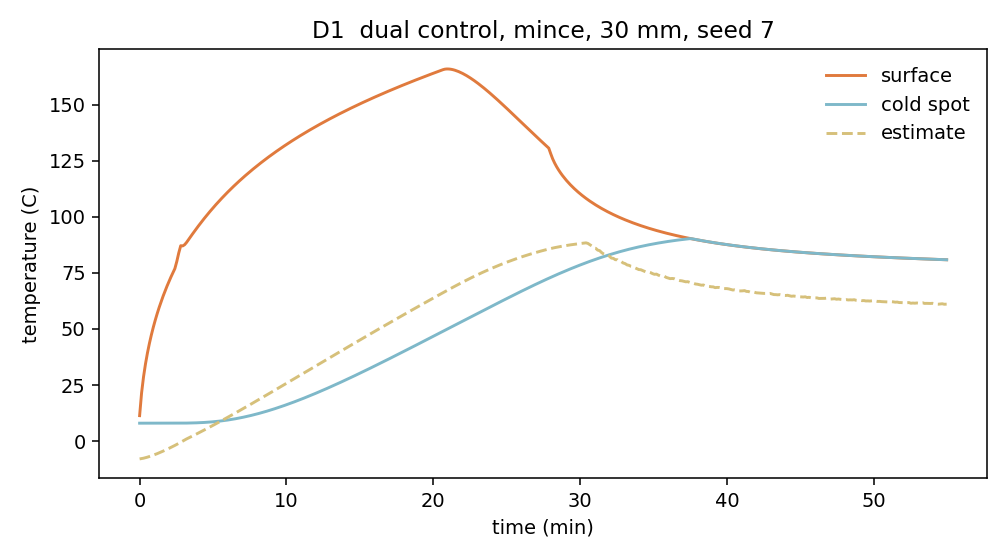
\includegraphics[width=0.86\textwidth]{D1_temperature.png}
\caption{D1。肉糜、30 mm、种子 7、对偶策略的表面温度、冷点温度和估计冷点，时间以分钟计。这是一条轨迹，不是中位数。它不能支持物理实验、二维脂肪几何或浏览器副本的温度。}
\end{figure}

\begin{figure}[ht]
\centering
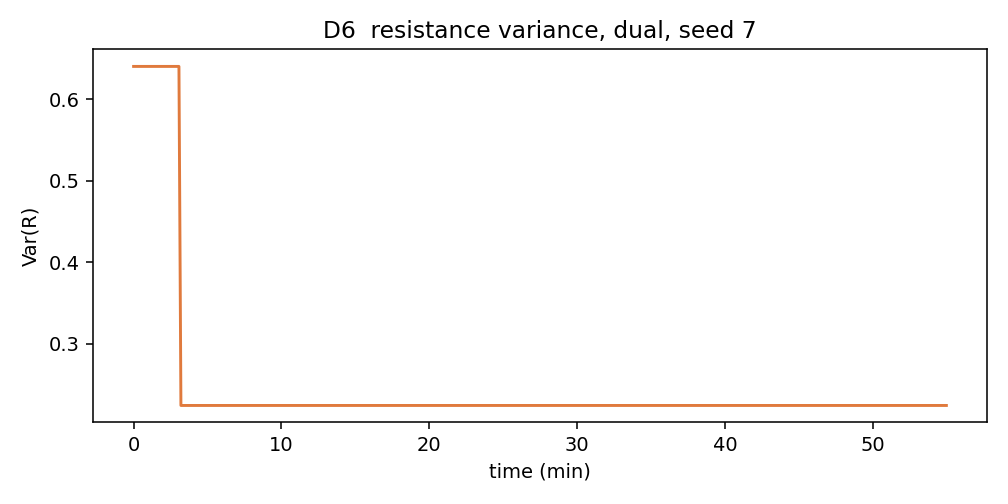
\includegraphics[width=0.86\textwidth]{D6_variance.png}
\caption{D6。同一条轨迹的热阻方差。192 s 处从 0.64 降到 0.224。降幅等于规则中的乘子 0.35，不是 Fisher 信息的特征值。不能据此比较 P0、P1、P2、P4。}
\end{figure}

\begin{figure}[ht]
\centering
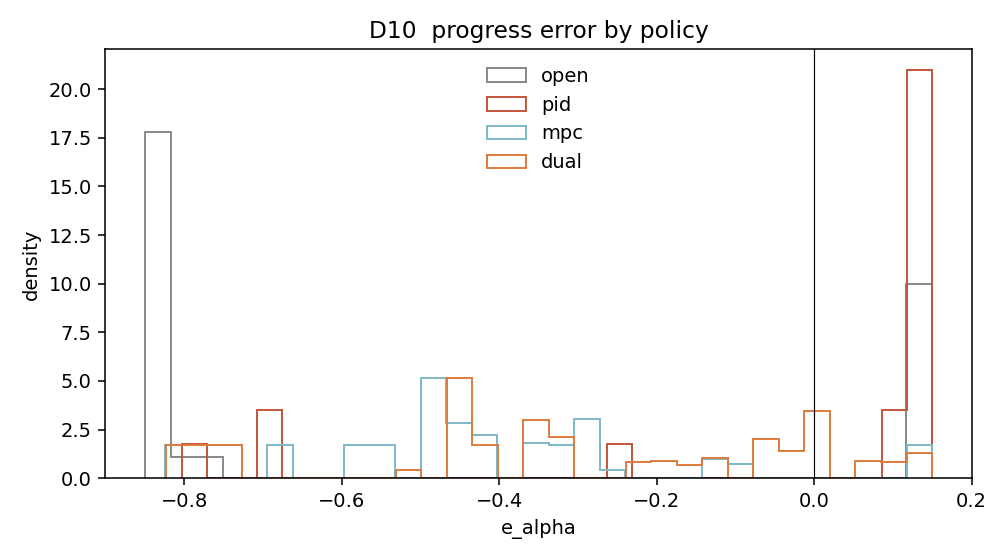
\includegraphics[width=0.86\textwidth]{D10_policy.png}
\caption{D10。四个策略的 \(e_{\alpha}\) 分布，每个策略 4860 条。零线是设计线。腔温比例的质量堆在 \(+0.15\)。这张图不能单独说明能耗，能耗在交叉表里，而且不能在没有 D10 的情况下单独作为结论。}
\end{figure}

\begin{figure}[ht]
\centering
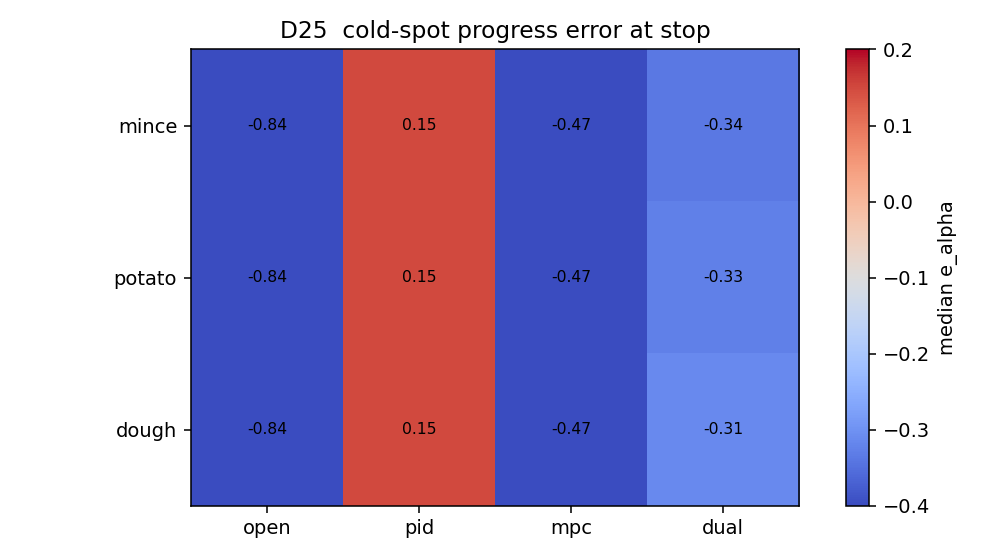
\includegraphics[width=0.86\textwidth]{D25_e_alpha.png}
\caption{D25。原型与策略的中位 \(e_{\alpha}\)。三个原型几乎相同，因为核里原型只改活度尺度。不能写成蛋白与淀粉的反应差异已经检验。}
\end{figure}

\begin{figure}[ht]
\centering
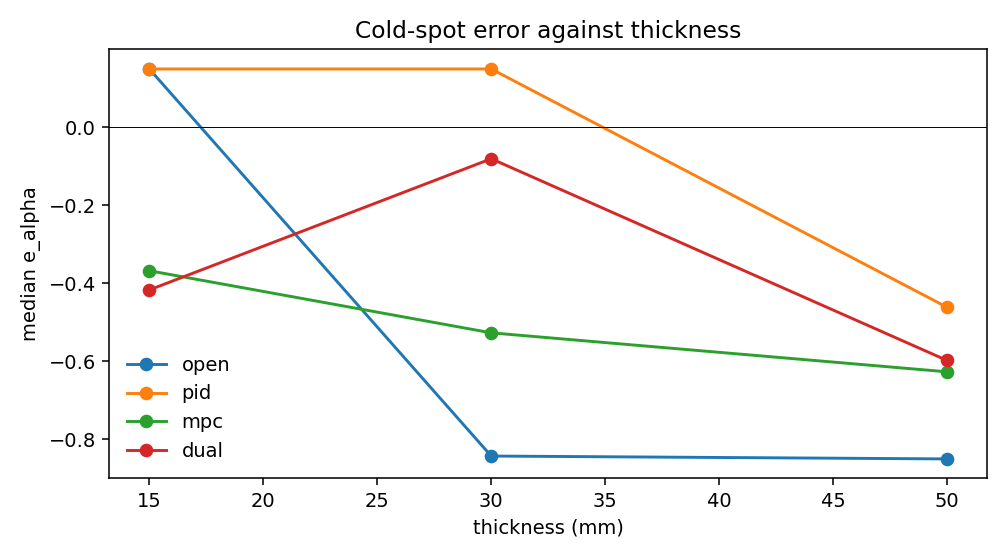
\includegraphics[width=0.86\textwidth]{D7_thickness.png}
\caption{D7。厚度与策略的进度误差。15 mm 的开环达到上沿；30 mm 的对偶中位数接近零而无探针仍明显为负；50 mm 两者都为负。不能外推到未运行的二维几何。}
\end{figure}

厚度把四个策略分开。箱线取自同一份摘要，离群点没有画出，所以须的端点是四分位以外的样本，不是全部样本的极值。

\begin{figure}[ht]
\centering
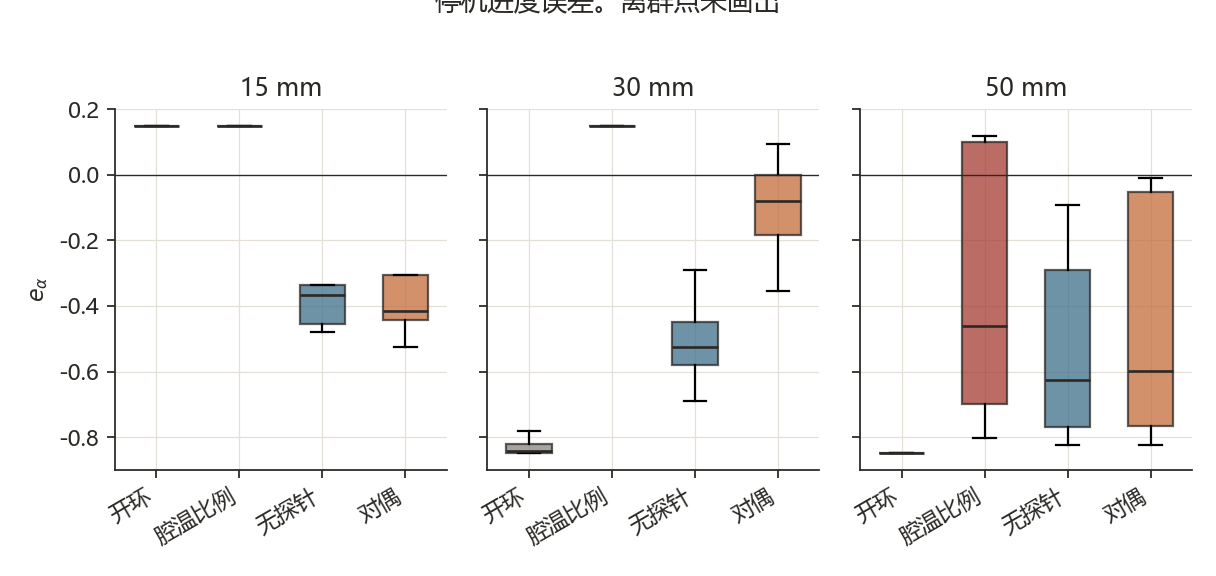
\includegraphics[width=\textwidth]{paper/P_box_thickness.png}
\caption{停机进度误差按厚度分开。15 mm 上对偶与无探针接近，开环和腔温比例贴在上沿。30 mm 上对偶的箱子跨过零线，无探针仍在零下。50 mm 上两者的中位数都在零下。腔温比例在 15 mm 与 30 mm 上贴住上沿，在 50 mm 上展开。}
\end{figure}

\begin{figure}[ht]
\centering
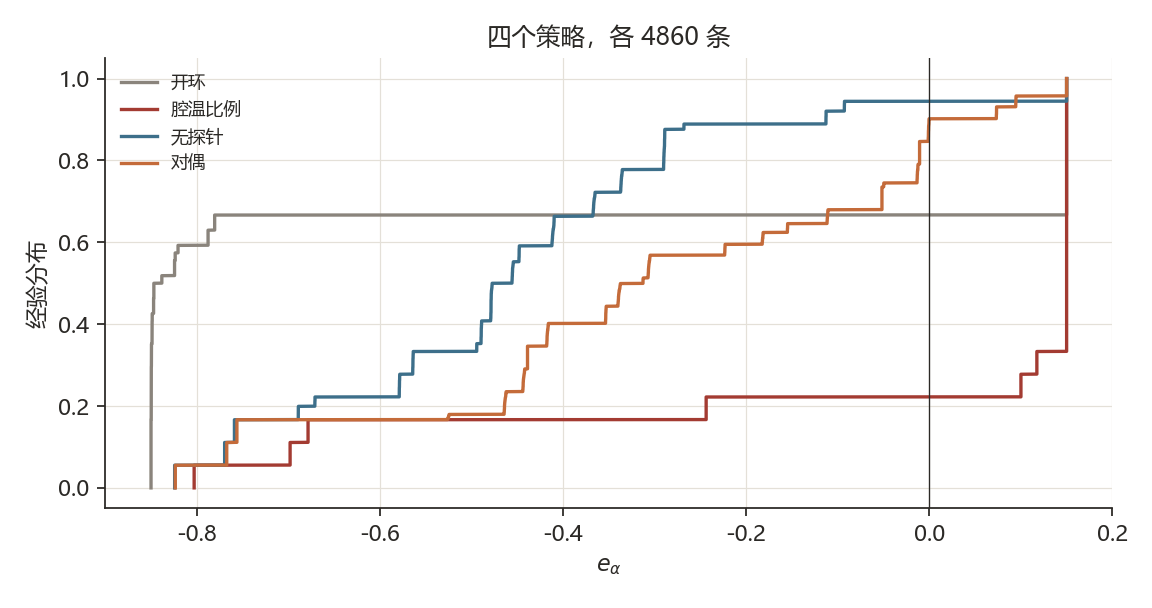
\includegraphics[width=0.92\textwidth]{paper/P_ecdf.png}
\caption{经验分布，每个策略 4860 条。零线是设计线。腔温比例在右端有一截竖起的质量，对应进度饱和。}
\end{figure}

\begin{figure}[ht]
\centering
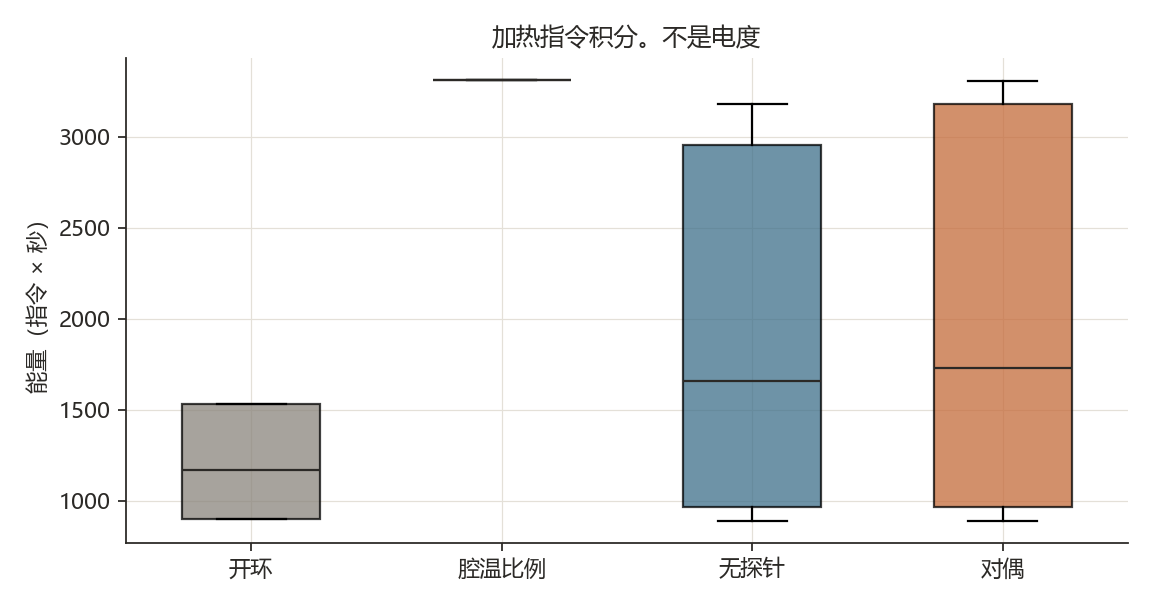
\includegraphics[width=0.86\textwidth]{paper/P_energy.png}
\caption{加热指令对记录间隔求和。开环最省，腔温比例最大。对偶略高于无探针。单位不是电度。}
\end{figure}

\begin{figure}[ht]
\centering
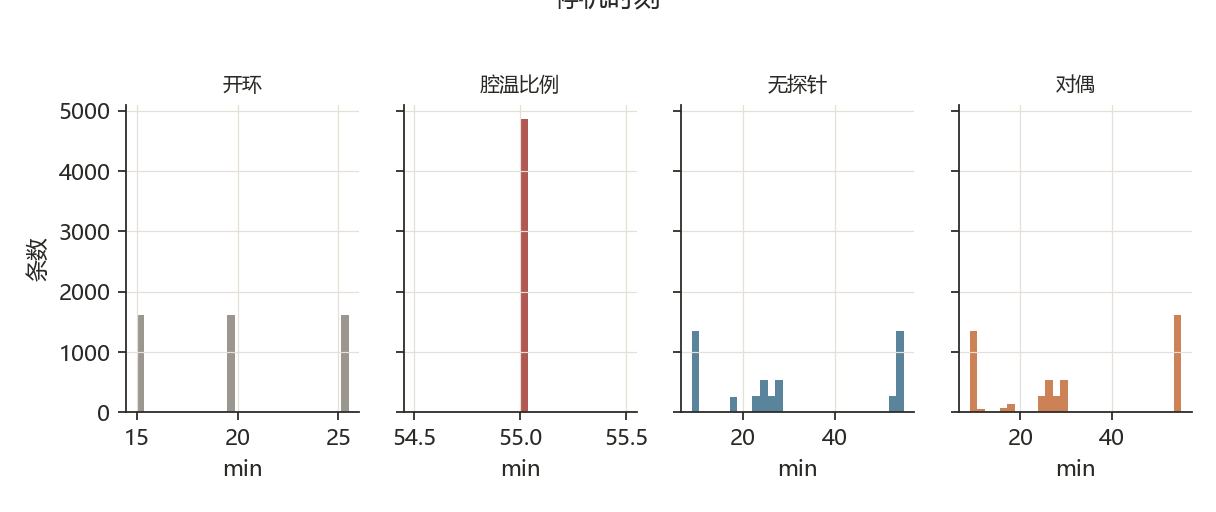
\includegraphics[width=\textwidth]{paper/P_stop.png}
\caption{停机时刻。开环集中在三档菜单时间。腔温比例全部停在时域终点。无探针与对偶的停机分布随厚度移动。}
\end{figure}

\begin{figure}[ht]
\centering
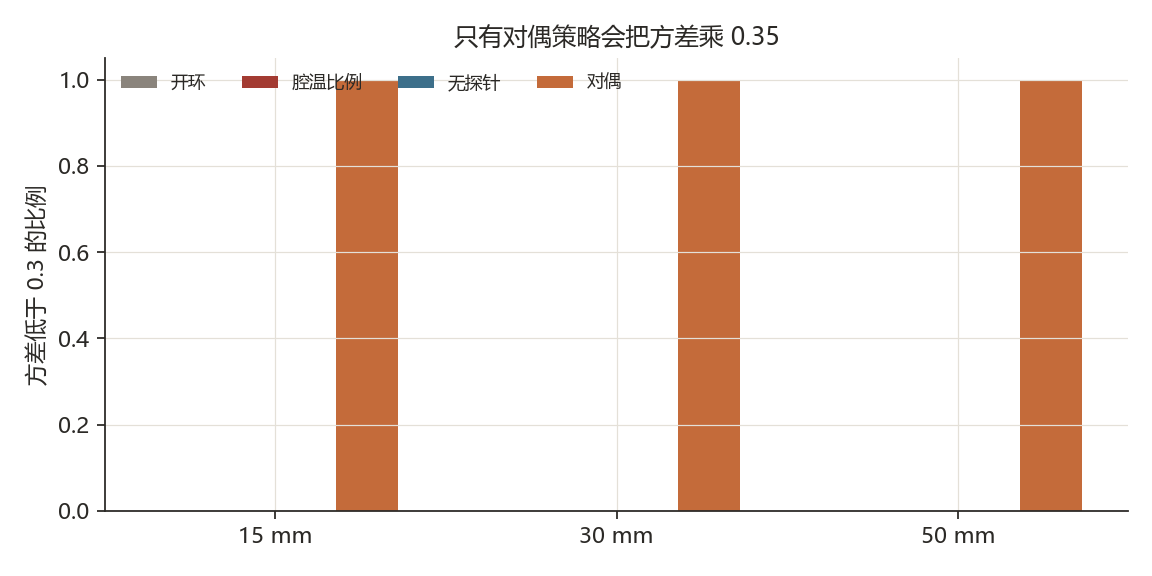
\includegraphics[width=0.86\textwidth]{paper/P_varr.png}
\caption{终点方差低于 0.3 的比例。只有对偶策略执行乘 0.35 的更新。另外三列是 0。}
\end{figure}

完整的分组中位数在下面的表里，来自同一份 \texttt{s1\_summary.json}。

\subsection{日志交叉表}
表中每一行来自 \texttt{s1\_summary.json} 的分组中位数与分位。$e$ 是停机时 $\alpha_m-0.85$。$e{<}0$ 表示停在设计线之下。$e_{50}=0.150$ 且上尾贴住 $0.150$，是进度饱和到 $1$ 之后的上沿，不是测量精度。能量 $E$ 是加热指令对时间的求和，单位为指令$\times$秒，不是电度。全部记录 \texttt{augmented=false}，\texttt{source=simulation}。这些行是同一数值核的样本，不是独立烹饪实验。
\begin{longtable}{lrrrrrrr}
\caption{四个策略的总体}\\
\toprule
分组 & $n$ & $e_{10}$ & $e_{50}$ & $e_{90}$ & $P(e{<}0)$ & $E_{50}$ & $t_{50}$ \\
\midrule
\endfirsthead
\toprule
分组 & $n$ & $e_{10}$ & $e_{50}$ & $e_{90}$ & $P(e{<}0)$ & $E_{50}$ & $t_{50}$ \\
\midrule
\endhead
dual & 4860 & -0.767 & -0.313 & -0.000 & 0.902 & 1730 & 1641 \\
mpc & 4860 & -0.770 & -0.467 & -0.113 & 0.944 & 1655 & 1540 \\
open & 4860 & -0.850 & -0.843 & 0.150 & 0.667 & 1170 & 1170 \\
pid & 4860 & -0.698 & 0.150 & 0.150 & 0.222 & 3310 & 3300 \\
\bottomrule
\end{longtable}

\begin{longtable}{lrrrrrrr}
\caption{食材与策略}\\
\toprule
分组 & $n$ & $e_{10}$ & $e_{50}$ & $e_{90}$ & $P(e{<}0)$ & $E_{50}$ & $t_{50}$ \\
\midrule
\endfirsthead
\toprule
分组 & $n$ & $e_{10}$ & $e_{50}$ & $e_{90}$ & $P(e{<}0)$ & $E_{50}$ & $t_{50}$ \\
\midrule
\endhead
dough, dual & 1620 & -0.767 & -0.313 & 0.007 & 0.900 & 1730 & 1641 \\
dough, mpc & 1620 & -0.770 & -0.467 & -0.113 & 0.944 & 1655 & 1540 \\
dough, open & 1620 & -0.850 & -0.836 & 0.150 & 0.667 & 1170 & 1170 \\
dough, pid & 1620 & -0.698 & 0.150 & 0.150 & 0.222 & 3310 & 3300 \\
mince, dual & 1620 & -0.767 & -0.338 & -0.000 & 0.904 & 1730 & 1641 \\
mince, mpc & 1620 & -0.770 & -0.467 & -0.113 & 0.944 & 1655 & 1540 \\
mince, open & 1620 & -0.850 & -0.843 & 0.150 & 0.667 & 1170 & 1170 \\
mince, pid & 1620 & -0.698 & 0.150 & 0.150 & 0.222 & 3310 & 3300 \\
potato, dual & 1620 & -0.767 & -0.325 & -0.000 & 0.902 & 1729 & 1641 \\
potato, mpc & 1620 & -0.770 & -0.467 & -0.113 & 0.944 & 1655 & 1540 \\
potato, open & 1620 & -0.850 & -0.836 & 0.150 & 0.667 & 1170 & 1170 \\
potato, pid & 1620 & -0.698 & 0.150 & 0.150 & 0.222 & 3310 & 3300 \\
\bottomrule
\end{longtable}

\begin{longtable}{lrrrrrrr}
\caption{厚度与策略}\\
\toprule
分组 & $n$ & $e_{10}$ & $e_{50}$ & $e_{90}$ & $P(e{<}0)$ & $E_{50}$ & $t_{50}$ \\
\midrule
\endfirsthead
\toprule
分组 & $n$ & $e_{10}$ & $e_{50}$ & $e_{90}$ & $P(e{<}0)$ & $E_{50}$ & $t_{50}$ \\
\midrule
\endhead
15.0, dual & 1620 & -0.464 & -0.417 & 0.150 & 0.872 & 932 & 591 \\
15.0, mpc & 1620 & -0.478 & -0.367 & 0.150 & 0.833 & 933 & 594 \\
15.0, open & 1620 & 0.150 & 0.150 & 0.150 & 0.000 & 900 & 900 \\
15.0, pid & 1620 & 0.150 & 0.150 & 0.150 & 0.000 & 3310 & 3300 \\
30.0, dual & 1620 & -0.353 & -0.080 & 0.073 & 0.833 & 1730 & 1641 \\
30.0, mpc & 1620 & -0.671 & -0.527 & -0.290 & 1.000 & 1655 & 1540 \\
30.0, open & 1620 & -0.849 & -0.843 & -0.780 & 1.000 & 1170 & 1170 \\
30.0, pid & 1620 & 0.150 & 0.150 & 0.150 & 0.000 & 3310 & 3300 \\
50.0, dual & 1620 & -0.823 & -0.598 & -0.011 & 1.000 & 3250 & 3300 \\
50.0, mpc & 1620 & -0.824 & -0.627 & -0.113 & 1.000 & 3055 & 3292 \\
50.0, open & 1620 & -0.850 & -0.850 & -0.850 & 1.000 & 1530 & 1530 \\
50.0, pid & 1620 & -0.803 & -0.461 & 0.117 & 0.667 & 3310 & 3300 \\
\bottomrule
\end{longtable}

\begin{longtable}{lrrrrrrr}
\caption{食材、厚度与策略}\\
\toprule
分组 & $n$ & $e_{10}$ & $e_{50}$ & $e_{90}$ & $P(e{<}0)$ & $E_{50}$ & $t_{50}$ \\
\midrule
\endfirsthead
\toprule
分组 & $n$ & $e_{10}$ & $e_{50}$ & $e_{90}$ & $P(e{<}0)$ & $E_{50}$ & $t_{50}$ \\
\midrule
\endhead
dough, 15.0, dual & 540 & -0.464 & -0.416 & 0.150 & 0.867 & 932 & 592 \\
dough, 15.0, mpc & 540 & -0.478 & -0.367 & 0.150 & 0.833 & 933 & 594 \\
dough, 15.0, open & 540 & 0.150 & 0.150 & 0.150 & 0.000 & 900 & 900 \\
dough, 15.0, pid & 540 & 0.150 & 0.150 & 0.150 & 0.000 & 3310 & 3300 \\
dough, 30.0, dual & 540 & -0.353 & -0.080 & 0.073 & 0.833 & 1730 & 1641 \\
dough, 30.0, mpc & 540 & -0.689 & -0.527 & -0.290 & 1.000 & 1655 & 1540 \\
dough, 30.0, open & 540 & -0.849 & -0.836 & -0.780 & 1.000 & 1170 & 1170 \\
dough, 30.0, pid & 540 & 0.150 & 0.150 & 0.150 & 0.000 & 3310 & 3300 \\
dough, 50.0, dual & 540 & -0.823 & -0.598 & -0.011 & 1.000 & 3250 & 3300 \\
dough, 50.0, mpc & 540 & -0.824 & -0.627 & -0.113 & 1.000 & 3053 & 3291 \\
dough, 50.0, open & 540 & -0.850 & -0.850 & -0.850 & 1.000 & 1530 & 1530 \\
dough, 50.0, pid & 540 & -0.803 & -0.461 & 0.117 & 0.667 & 3310 & 3300 \\
mince, 15.0, dual & 540 & -0.464 & -0.417 & 0.150 & 0.878 & 932 & 591 \\
mince, 15.0, mpc & 540 & -0.478 & -0.367 & 0.150 & 0.833 & 933 & 594 \\
mince, 15.0, open & 540 & 0.150 & 0.150 & 0.150 & 0.000 & 900 & 900 \\
mince, 15.0, pid & 540 & 0.150 & 0.150 & 0.150 & 0.000 & 3310 & 3300 \\
mince, 30.0, dual & 540 & -0.353 & -0.080 & 0.073 & 0.833 & 1730 & 1641 \\
mince, 30.0, mpc & 540 & -0.671 & -0.527 & -0.290 & 1.000 & 1655 & 1540 \\
mince, 30.0, open & 540 & -0.850 & -0.843 & -0.821 & 1.000 & 1170 & 1170 \\
mince, 30.0, pid & 540 & 0.150 & 0.150 & 0.150 & 0.000 & 3310 & 3300 \\
mince, 50.0, dual & 540 & -0.823 & -0.598 & -0.011 & 1.000 & 3250 & 3300 \\
mince, 50.0, mpc & 540 & -0.824 & -0.627 & -0.113 & 1.000 & 3055 & 3292 \\
mince, 50.0, open & 540 & -0.850 & -0.850 & -0.850 & 1.000 & 1530 & 1530 \\
mince, 50.0, pid & 540 & -0.803 & -0.461 & 0.117 & 0.667 & 3310 & 3300 \\
potato, 15.0, dual & 540 & -0.464 & -0.417 & 0.150 & 0.872 & 932 & 591 \\
potato, 15.0, mpc & 540 & -0.478 & -0.367 & 0.150 & 0.833 & 933 & 594 \\
potato, 15.0, open & 540 & 0.150 & 0.150 & 0.150 & 0.000 & 900 & 900 \\
potato, 15.0, pid & 540 & 0.150 & 0.150 & 0.150 & 0.000 & 3310 & 3300 \\
potato, 30.0, dual & 540 & -0.353 & -0.080 & 0.073 & 0.833 & 1729 & 1641 \\
potato, 30.0, mpc & 540 & -0.671 & -0.527 & -0.290 & 1.000 & 1655 & 1540 \\
potato, 30.0, open & 540 & -0.849 & -0.836 & -0.780 & 1.000 & 1170 & 1170 \\
potato, 30.0, pid & 540 & 0.150 & 0.150 & 0.150 & 0.000 & 3310 & 3300 \\
potato, 50.0, dual & 540 & -0.823 & -0.598 & -0.011 & 1.000 & 3249 & 3300 \\
potato, 50.0, mpc & 540 & -0.824 & -0.627 & -0.113 & 1.000 & 3055 & 3292 \\
potato, 50.0, open & 540 & -0.850 & -0.850 & -0.850 & 1.000 & 1530 & 1530 \\
potato, 50.0, pid & 540 & -0.803 & -0.461 & 0.117 & 0.667 & 3310 & 3300 \\
\bottomrule
\end{longtable}

\begin{longtable}{lrrrrrrr}
\caption{非均质档、厚度与策略}\\
\toprule
分组 & $n$ & $e_{10}$ & $e_{50}$ & $e_{90}$ & $P(e{<}0)$ & $E_{50}$ & $t_{50}$ \\
\midrule
\endfirsthead
\toprule
分组 & $n$ & $e_{10}$ & $e_{50}$ & $e_{90}$ & $P(e{<}0)$ & $E_{50}$ & $t_{50}$ \\
\midrule
\endhead
0, 15.0, dual & 540 & -0.444 & -0.391 & -0.338 & 1.000 & 924 & 578 \\
0, 15.0, mpc & 540 & -0.479 & -0.422 & -0.365 & 1.000 & 925 & 580 \\
0, 15.0, open & 540 & 0.150 & 0.150 & 0.150 & 0.000 & 900 & 900 \\
0, 15.0, pid & 540 & 0.150 & 0.150 & 0.150 & 0.000 & 3310 & 3300 \\
0, 30.0, dual & 540 & -0.155 & -0.080 & -0.013 & 1.000 & 1714 & 1617 \\
0, 30.0, mpc & 540 & -0.579 & -0.513 & -0.410 & 1.000 & 1640 & 1516 \\
0, 30.0, open & 540 & -0.849 & -0.835 & -0.788 & 1.000 & 1170 & 1170 \\
0, 30.0, pid & 540 & 0.150 & 0.150 & 0.150 & 0.000 & 3310 & 3300 \\
0, 50.0, dual & 540 & -0.767 & -0.409 & -0.052 & 1.000 & 3229 & 3300 \\
0, 50.0, mpc & 540 & -0.770 & -0.529 & -0.268 & 1.000 & 3024 & 3249 \\
0, 50.0, open & 540 & -0.850 & -0.850 & -0.850 & 1.000 & 1530 & 1530 \\
0, 50.0, pid & 540 & -0.698 & -0.299 & 0.100 & 0.500 & 3310 & 3300 \\
1, 15.0, dual & 540 & -0.418 & -0.362 & -0.305 & 1.000 & 931 & 583 \\
1, 15.0, mpc & 540 & -0.456 & -0.352 & -0.336 & 1.000 & 932 & 584 \\
1, 15.0, open & 540 & 0.150 & 0.150 & 0.150 & 0.000 & 900 & 900 \\
1, 15.0, pid & 540 & 0.150 & 0.150 & 0.150 & 0.000 & 3310 & 3300 \\
1, 30.0, dual & 540 & -0.001 & 0.036 & 0.095 & 0.500 & 1741 & 1643 \\
1, 30.0, mpc & 540 & -0.489 & -0.390 & -0.289 & 1.000 & 1664 & 1539 \\
1, 30.0, open & 540 & -0.849 & -0.834 & -0.780 & 1.000 & 1170 & 1170 \\
1, 30.0, pid & 540 & 0.150 & 0.150 & 0.150 & 0.000 & 3310 & 3300 \\
1, 50.0, dual & 540 & -0.756 & -0.383 & -0.011 & 1.000 & 3255 & 3300 \\
1, 50.0, mpc & 540 & -0.759 & -0.436 & -0.093 & 1.000 & 3071 & 3281 \\
1, 50.0, open & 540 & -0.850 & -0.850 & -0.850 & 1.000 & 1530 & 1530 \\
1, 50.0, pid & 540 & -0.678 & -0.280 & 0.117 & 0.500 & 3310 & 3300 \\
2, 15.0, dual & 540 & -0.525 & -0.463 & 0.150 & 0.617 & 941 & 607 \\
2, 15.0, mpc & 540 & -0.412 & -0.130 & 0.150 & 0.500 & 988 & 799 \\
2, 15.0, open & 540 & 0.150 & 0.150 & 0.150 & 0.000 & 900 & 900 \\
2, 15.0, pid & 540 & 0.150 & 0.150 & 0.150 & 0.000 & 3310 & 3300 \\
2, 30.0, dual & 540 & -0.353 & -0.268 & -0.182 & 1.000 & 1749 & 1670 \\
2, 30.0, mpc & 540 & -0.689 & -0.618 & -0.564 & 1.000 & 1674 & 1568 \\
2, 30.0, open & 540 & -0.850 & -0.844 & -0.824 & 1.000 & 1170 & 1170 \\
2, 30.0, pid & 540 & 0.150 & 0.150 & 0.150 & 0.000 & 3310 & 3300 \\
2, 50.0, dual & 540 & -0.823 & -0.631 & -0.439 & 1.000 & 3245 & 3300 \\
2, 50.0, mpc & 540 & -0.824 & -0.659 & -0.479 & 1.000 & 3066 & 3292 \\
2, 50.0, open & 540 & -0.850 & -0.850 & -0.850 & 1.000 & 1530 & 1530 \\
2, 50.0, pid & 540 & -0.803 & -0.523 & -0.244 & 1.000 & 3310 & 3300 \\
\bottomrule
\end{longtable}

\begin{longtable}{lrrrrrrr}
\caption{初始含水与策略}\\
\toprule
分组 & $n$ & $e_{10}$ & $e_{50}$ & $e_{90}$ & $P(e{<}0)$ & $E_{50}$ & $t_{50}$ \\
\midrule
\endfirsthead
\toprule
分组 & $n$ & $e_{10}$ & $e_{50}$ & $e_{90}$ & $P(e{<}0)$ & $E_{50}$ & $t_{50}$ \\
\midrule
\endhead
0.64, dual & 1620 & -0.767 & -0.313 & -0.000 & 0.902 & 1730 & 1641 \\
0.64, mpc & 1620 & -0.770 & -0.467 & -0.113 & 0.944 & 1655 & 1540 \\
0.64, open & 1620 & -0.850 & -0.843 & 0.150 & 0.667 & 1170 & 1170 \\
0.64, pid & 1620 & -0.698 & 0.150 & 0.150 & 0.222 & 3310 & 3300 \\
0.72, dual & 1620 & -0.767 & -0.313 & -0.000 & 0.902 & 1730 & 1641 \\
0.72, mpc & 1620 & -0.770 & -0.467 & -0.113 & 0.944 & 1655 & 1540 \\
0.72, open & 1620 & -0.850 & -0.843 & 0.150 & 0.667 & 1170 & 1170 \\
0.72, pid & 1620 & -0.698 & 0.150 & 0.150 & 0.222 & 3310 & 3300 \\
0.8, dual & 1620 & -0.767 & -0.313 & -0.000 & 0.902 & 1730 & 1641 \\
0.8, mpc & 1620 & -0.770 & -0.467 & -0.113 & 0.944 & 1655 & 1540 \\
0.8, open & 1620 & -0.850 & -0.843 & 0.150 & 0.667 & 1170 & 1170 \\
0.8, pid & 1620 & -0.698 & 0.150 & 0.150 & 0.222 & 3310 & 3300 \\
\bottomrule
\end{longtable}

\begin{longtable}{lrrrrrrr}
\caption{初始温度与策略}\\
\toprule
分组 & $n$ & $e_{10}$ & $e_{50}$ & $e_{90}$ & $P(e{<}0)$ & $E_{50}$ & $t_{50}$ \\
\midrule
\endfirsthead
\toprule
分组 & $n$ & $e_{10}$ & $e_{50}$ & $e_{90}$ & $P(e{<}0)$ & $E_{50}$ & $t_{50}$ \\
\midrule
\endhead
5.0, dual & 2430 & -0.823 & -0.417 & -0.000 & 0.915 & 1822 & 1740 \\
5.0, mpc & 2430 & -0.824 & -0.579 & 0.150 & 0.889 & 1738 & 1628 \\
5.0, open & 2430 & -0.850 & -0.849 & 0.150 & 0.667 & 1170 & 1170 \\
5.0, pid & 2430 & -0.803 & 0.150 & 0.150 & 0.333 & 3310 & 3300 \\
20.0, dual & 2430 & -0.463 & -0.182 & 0.073 & 0.889 & 1658 & 1544 \\
20.0, mpc & 2430 & -0.564 & -0.366 & -0.113 & 1.000 & 1587 & 1448 \\
20.0, open & 2430 & -0.850 & -0.821 & 0.150 & 0.667 & 1170 & 1170 \\
20.0, pid & 2430 & -0.244 & 0.150 & 0.150 & 0.111 & 3310 & 3300 \\
\bottomrule
\end{longtable}


读表时只增加图里没有写完的比较。初始含水三档和初温两档没有改变策略排序的方向：厚度仍然是主因子。非均质档 2 把一个控制体的导热降低，厚件的提前没有因此消失。表中的能量单位是加热指令乘以记录间隔，不是电度。停止时刻的中位数与菜单时间在开环上重合：15 mm 为 900 s，30 mm 为 1170 s，50 mm 为 1530 s，说明开环确实停在菜单终点。

\subsection{能量、方差与褐变}
下列数字由 \texttt{s1\_summary.json} 的 19440 行重新分组。能量仍是加热指令乘记录间隔。方差低于 0.3 表示走过一次乘 0.35 的更新；未更新的先验方差是 0.64。褐变是终点 $\alpha_b$，不是停机时刻。
\begin{longtable}{lrrrrrr}
\caption{按厚度与策略的能量分位与终点方差}\\
\toprule
分组 & $n$ & $E_{10}$ & $E_{50}$ & $E_{90}$ & 方差$<0.3$ & $\alpha_{b,50}$ \\
\midrule\endfirsthead
\toprule 分组 & $n$ & $E_{10}$ & $E_{50}$ & $E_{90}$ & 方差$<0.3$ & $\alpha_{b,50}$ \\\midrule\endhead
15\,mm, 开环 & 1620 & 900 & 900 & 900 & 0.000 & 0.0000 \\
15\,mm, 腔温比例 & 1620 & 3310 & 3310 & 3310 & 0.000 & 0.0000 \\
15\,mm, 无探针 & 1620 & 892 & 933 & 1076 & 0.000 & 0.0000 \\
15\,mm, 对偶 & 1620 & 890 & 932 & 1064 & 1.000 & 0.0000 \\
30\,mm, 开环 & 1620 & 1170 & 1170 & 1170 & 0.000 & 0.0000 \\
30\,mm, 腔温比例 & 1620 & 3310 & 3310 & 3310 & 0.000 & 0.0000 \\
30\,mm, 无探针 & 1620 & 1563 & 1655 & 1753 & 0.000 & 0.0000 \\
30\,mm, 对偶 & 1620 & 1629 & 1730 & 1836 & 1.000 & 0.0000 \\
50\,mm, 开环 & 1620 & 1530 & 1530 & 1530 & 0.000 & 0.0000 \\
50\,mm, 腔温比例 & 1620 & 3310 & 3310 & 3310 & 0.000 & 0.0000 \\
50\,mm, 无探针 & 1620 & 2901 & 3055 & 3178 & 0.000 & 0.0000 \\
50\,mm, 对偶 & 1620 & 3157 & 3250 & 3307 & 1.000 & 0.0000 \\
\bottomrule\end{longtable}
对偶在三档厚度上的方差下降比例都是 1。开环、腔温比例和无探针的比例是 0，因为它们的代码路径不写 $\hat r$。终点褐变的中位数在这十二格里都是 0：表面含水没有降到褐变式要求的 0.55 以下，或者表面温度没有同时越过 $110^\circ\mathrm{C}$。中位数为 0 不表示每一条轨迹的 $\alpha_b$ 都是 0。三个原型在 S1 的含水格子上活度都贴近饱和，所以这张表也不能比较蛋白与淀粉的表面反应。


\paragraph{本节不能推出的结论}
表中任何一格都是数值样本。它不能出现在以“实验验证”为谓语的句子里。终点褐变中位数为 0，不能写成表面品质已经比较过。

\section{软件结构}

规格中的目录把真值步进、传感器、估计、探针、孪生、预测控制、算子和评价分开，评价与控制不共享内存中的真值对象。本次实现没有这些目录。积分、策略和评分在同一次循环里。评价能做的隔离只有：摘要文件在循环之后读取，图从摘要和一条演示轨迹生成。浏览器副本不读这份摘要。

噪声用正弦散列，不用随机数发生器，所以同一版本的代码重复运行得到同一日志。策略编号进入散列的相位，四个策略的噪声实现不相同。

\paragraph{本节不能推出的结论}
代码可复现，不能推出格式误差已经通过 S0。网格减半没有做。

\section{几何保真度的三档}

\begin{table}[ht]
\centering
\caption{几何档与本次归属}
\begin{tabularx}{\textwidth}{llX}
\toprule
档 & 规格 & 本次 \\
\midrule
T1 & 一维全因子，策略排序的主表 & 十六条控制体已运行，作为本章全部数字的归属 \\
T2 & 二维截面，脂肪夹层与各向异性 & 未运行。不能用档 2 的一个低导热控制体代替 \\
T3 & 风速与蒸汽的外部流动，只提供边界库 & 未运行。\(h\) 是线性式 \\
\bottomrule
\end{tabularx}
\end{table}

在线集合 32 与离线 128 没有运行。神经算子没有用 T1 训练，也没有在 T2 上做干预测试。一维结果不外推为整机三维热场。三维全耦合不在本章的结论内。

\paragraph{本章不能推出的结论}
主结论只限于：在这个一维核上，按厚度分开看，开环该薄的过了、该厚的没到；腔温比例靠持续加热把进度推到上沿，厚件仍有三分之二提前；无探针经常在真值进度未到设计线时停止；对偶在 30 mm 上把中位误差从约 \(-0.53\) 拉到约 \(-0.08\)，在 15 mm 上没有优势，在 50 mm 上两者都提前。这些句子的主语都是本核。它们不是多孔介质真值、不是集合滤波、也不是预测控制求解器的结果。
